%-------------------- begin preamble ----------------------

\documentclass
[twocolumn,
secnumarabic,
nobibnotes,
aps,
prl,
reprint,
groupedaddress,
amsmath,
amssymb
]{revtex4-2}

\usepackage{relsize,makeidx,color,setspace,amsfonts}

\usepackage{listings}
\lstset{
    language=Python,
    inputencoding=utf8,
    extendedchars=true,
    literate={ø}{{\o}}1 {å}{{\r a}}1 {Å}{{\r A}}1 {æ}{{\ae}}1,
    backgroundcolor=\color{white},
    basicstyle=\footnotesize\ttfamily,
    breakatwhitespace=false,
    breaklines=true,
    captionpos=b,
    commentstyle=\itshape\color{purple!60!black},
    frame=single,
    %identifierstyle=\color{orange},
    keepspaces=true,
    keywordstyle=\bfseries\color{violet},
    numbers=left,
    numbersep=5pt,
    numberstyle=\tiny\color{black},
    rulecolor=\color{black},
    showstringspaces=false,
    showtabs=false,
    stepnumber=1,
    stringstyle=\color{purple!60!black},
    tabsize=2,
    title=\lstname
  }
\usepackage{dcolumn}% Align table columns on decimal point
\usepackage[table]{xcolor}
\usepackage{bm,ltablex,microtype}
\usepackage{longtable}
\usepackage{siunitx}
\usepackage{algorithm2e}
\usepackage{csvsimple}
\usepackage{url}
\renewcommand{\UrlFont}{\small\tt}

\usepackage[pdftex]{graphicx}

\usepackage{fancyvrb} % packages needed for verbatim environments

\usepackage[T1]{fontenc}

\usepackage{ucs}
\usepackage[utf8]{inputenc}

\usepackage{lmodern}         % Latin Modern fonts derived from Computer Modern

% Hyperlinks in PDF:
\definecolor{linkcolor}{rgb}{0,0,0}
\usepackage{hyperref}
\hypersetup{
breaklinks=true,
colorlinks=true,
linkcolor=linkcolor,
urlcolor=linkcolor,
citecolor=black,
filecolor=black,
%filecolor=blue,
pdfmenubar=true,
pdftoolbar=true,
bookmarksdepth=3   % Uncomment (and tweak) for PDF bookmarks with more levels than the TOC
}


\setcounter{tocdepth}{2}  % levels in table of contents

% prevent orhpans and widows
\clubpenalty = 10000
\widowpenalty = 10000

% --- end of standard preamble for documents ---

% insert custom LaTeX commands...

\raggedbottom
\makeindex
\setlength{\textheight}{9.5in}


%-------------------- end preamble ----------------------

\begin{document}

% ------------------- main content ----------------------

\title{FYS-STK4155 - Project2 TITLE SHOULD BE DESCRIPTIVE}

\author{Gard}
\author{Are}
\email{afkvanum@mail.uio.no}
\affiliation{Department of Geoscience, University of Oslo}
\author{David Andreas Bordvik}
\affiliation{Department of Informatics, University of Oslo}
\date{\today}

\begin{abstract}
  This will be our wonderfully conclusive abstract
\end{abstract}

\maketitle

\section{Introduction}
Feed-Forward Neural Networks takes the idea of connecting artificial neurons in layers to create a fully connected network. Information flows in a single direction through the network, from the input layer to the evaluation of the input in the output layer. A Feed-Forward network can be used to approximate a function. The network does this by learning which parameters, given some input, results in the closest representation of the correct output \cite{Goodfellow2016}.

The \textbf{Universal approximation theorem} states that a Neural Network can approximate any function with as few as a single hidden layer to any precision \cite{Hornik1989, Cybenko1989}. Hence, any feedforward network with a single hidden layer is in theory ample to represent any function, due to their underlying universality \cite{Nielsen2015}. For this project, we will use the \textbf{Universal approximation theorem} as motivation to develop our own Feed-Forward Neural Network code to study both classification and regression.

When studying regression using our developed Feed-Forward Neural Network code, we will return to the terrain data used in Project 1 when studying polynomial fitting with different variants of Least Squares Regression. Moreover, we will compare our findings in this project with the result of our previous project to further study the differences polynomial fitting and gradient based approximations. 

Furthermore, we will study classification using the \href{https://www.kaggle.com/uciml/breast-cancer-wisconsin-data}{Wisconsin Breast Cancer Data} provided by SciKit-learn \cite{scikit-learn}. When studying the accuracy of the Neural Net in the context of classification, we will also develop code for Logistic Regression for comparison.

The following sections will include background theory and proposals to algorithms which will be needed to construct our Feed-Forward Neural Network. All algorithms developed will be discussed in detail, however for the concrete implementation we refer to the GitHub repository linked in the Appendix under the section Source Code.

For clarity, all source code developed has been written using the Python programming language. Results obtained from our own developed code will also be compared to functions from the Machine Learning libraries SciKit-Learn \cite{scikit-learn}, PyTorch \cite{paszke2019} and TensorFlow \cite{tensorflow2015-whitepaper}.

In the following section, we will derive the theory and develop an algorithm for Stochastic Gradient Descent. Using that algorithm as a basis, we will further derive theory and develop code for our own Neural Network and Logistic Regression. With the developed algorithms, we will study their behavior and skill when used with both the Terrain data from Project 1 as well as the Breast Cancer data provided by SciKit-learn \cite{scikit-learn}. The results obtained from our own developed code, as well as the benchmarks with the previously stated Machine Learning software will be presented in the \textbf{Results} section. A discussion of our results will be confined to the \textbf{Discussion} section. Finally, the project will be concluded with our final thoughts for the results as well as this project as a whole in the \textbf{Conclusions} section.  

\section{Theory and Methods}
\subsection{Moving along the gradient}
Gradient Descent is an iterative algorithm that minimizes a given function by following its gradient down towards the global minimum. For a given cost-function $C(\beta)$ with predictors $\beta$ and a hyperparameter $\eta$ (which will be described in the following paragraph), the process of Gradient Descent can be expressed mathematically as follows
\begin{equation}
  \label{eq:gd}
  \beta_{k+1} = \beta_k - \eta\nabla_\beta\left(C(\beta_k)\right)
\end{equation}

By inspecting Equation (\ref{eq:gd}), it can be seen that given some random initialization of $\beta_0$, each step $\beta_k$ will be closer to the optimal $\hat{\beta}$ than the previous step. This is done by repeatedly calculating the cost function and taking a step in the direction of its gradient. Moreover, the length of the step taken is decided by the newly introduced hyperparameter $\eta$. Where consecutively large values of $\eta$ results in a large step along the gradient, and a small value of $\eta$ a small step along the gradient. The learning rate is an essential parameter to ensure that the gradient descent converges, as small values might end up slow convergence and large values result in divergence \cite{Geron2019}. 

Another pitfall for gradient based convergence methods is the existence of local minimums. As not all functions are created equal, some functions might feature some unevenness that the gradient descent will mistake as a global minimum. As such, gradient descent on the form as in Equation (\ref{eq:gd}) will get stuck in any local minima that it encounters. However, given the case of regression, the MSE cost function is a convex function. As such, there is only one minimum of the function which is the global minimum \cite{Geron2019}. Thus, when considering regression, there is no risk of the algorithm getting stuck in a local minima.

\subsection{Introducing stochasticity to gradient descent}
By utilizing the entire gradient of the cost function to compute the next step along the gradient, a lot of computational resources are utilized. Especially if one are to consider a large data-set consisting of several data-points and features. A method to alleviate some of the computational demand of the algorithm is to only compute the gradient for a smaller subset of the data. With Stochastic Gradient Descent, this idea is implemented with a stochastic element, that is, which subset of the data is used is selected at random. The resulting gradient algorithm converges towards the same global minimum as regular gradient descent over the entire data-set, though at a higher pace following an uneven gradient path \cite{Geron2019}.

Another benefit of Stochastic Gradient Descent (SGD) compared to its non-stochastic variant is its ability to exit local minima. As the SGD never reaches a true minimum, a local minima might not be able to contain the algorithm when recomputing the gradient based on a different subset of data. On the other hand, as a consequence of never achieving true minimum, SGD will never return optimal values when compared to non-stochastic gradient descent.

\subsubsection{Scheduling the learning rate}
As pointed out, the Stochastic Gradient Descent algorithm never achieves a minima, thus in effect the algorithm will always move until a set number of epochs has been reached. To simulate a stopping behavior of the algorithm, a learning rate scheduler which dynamically changes the learning rate can be implemented. In the context of this project, a scheduler which reduces the learning rate over time will be implemented.
The effect of reducing the learning rate over time is that the step length taken along the gradient after several epochs is smaller. Furthermore, Stochastic Gradient Descent might benefit from such a dynamic learning rate, as it can  be assumed that the algorithm have already closed in on convergence before reaching maximum number of epochs. The scheduler in turn will then be able to dampen all future steps taken, to minimize the effect of the random walk behaviour of the algorithm around the minima.
For our SGD algorithm, the learning rate scheduler we have implemented is an inverse scaling similarly to the \textit{invscaling} parameter passed on to SciKit-learn's \textbf{SGDRegressor} class. That is, the scheduler updates the learning rate following the equation $\eta = \eta_0/t^{t_0}$ \cite{scikit-learn}. However, in an attempt to reduce the immediate impact of the learning rate scheduler, the first 10 epochs will be completed without scheduling.

\subsection{Implementing Stochastic Gradient Descent}
By introducing the concept of mini-batches to Gradient Descent, we have to split our data randomly into mini-batches such that the resulting design matrix is 
$$
X_{\text{perm}} = \left\{X_0, X_1, \ldots, X_M\right\}^T
$$
where $M$ represents the number of mini-batches. Moreover, $X_i$ contains randomly drawn rows from $X$. The random draw can be both with and without replacement. In the case of the prior, some minibatches can be reused while others are skipped in their entirety. Whereas in the latter case, all minibatches have to be used to constitute one epoch. The difference between these implementations of Stochastic Gradient Descent is that the prior version with replacement tends to converge somewhat faster than the version without replacement \cite{Geron2019}. Furthermore, the target vector $t$ is shuffled in such a way that the rows in $X_{\text{perm}}$ still adheres to the same target $t_i$.

With the construction of $X_\text{perm}$, the algorithm moves forward by computing the gradient and moving along its direction one mini-batch at a time. Traversing through all mini-batches or a set number of them constitutes to one epoch. The algorithm just described is then rerun for a specified number of epochs.

The gradient step can be described mathematically as follows in Equation (\ref{eq:grad_step})
\begin{equation}\label{eq:grad_step}
  \beta_{j+1} = \beta_j - \eta_j\sum_{i \in B_k}^n\nabla_\beta c_i(\bm{x}_i,\beta_j)
\end{equation}
Stochastic Gradient Descent is implemented as pseudocode in Algorithm (\ref{alg:sgd})

\begin{algorithm}
  \SetAlgoLined
  \KwData{Design Matrix (X), target array (t) and initial guess at predictors $\theta$}
  \KwResult{Estimated value of the predictors $\theta$}
  \For{epoch in number of epochs}{
    \For{batch in number of batches}{
      $x_i \leftarrow$ X[batch]\;
      $t_i \leftarrow$ t[batch]\;
      Compute $\nabla_\theta{}C(\theta)$ with respect to $x_i$ and $t_i$\;
      $\eta \leftarrow learning_schedule(\eta, \ldots)$\;
      $\theta \leftarrow \theta - \eta*\nabla_\theta C(\theta)$\;
    }
  }
  \Return{$\theta$}
  \caption{\label{alg:sgd}Stochastic Gradient Descent with minibatches and learning rate scheduler}
\end{algorithm}

\subsection{Adding momentum to SGD}
Equation (\ref{eq:grad_step}) can be generalized with a momentum term as follows 

\begin{equation}
  \label{eq:momentum_grad}
  \begin{aligned}
    \bm{v}_t = \gamma\bm{v}_{t-1} + \eta_y\nabla_\theta E(\bm{\theta}_t) \\
    \bm{\theta}_{t+1} = \bm{\theta}_t - \bm{v}_t
  \end{aligned}
\end{equation}

Where the momentum parameter $\gamma \in \left[0,1\right]$. The intuition behind the introduction of the momentum parameter is the drag coefficient used in mechanics to describe friction. It's usage is similar when introduced in Stochastic Gradient Descent, as the momentum parameter enables the possibility for the gradient to attain momentum when traversing along a slope. Eventually if the gradient is ascending a gradient, due to the momentum, it might stop and return back down towards the minima. Thus Stochastic Gradient Descent with momentum enables the gradient to traverse through some local minima, while eventually stopping at the global minima. The algorithmic implementation of Momentum Stochastic Gradient Descent can be seen in Algorithm (\ref{alg:msgd}).

\begin{algorithm}
  \KwData{Design Matrix (X), target array (t) and initial guess at predictors $\theta$}
  \KwResult{Estimated value of the predictors $\theta$}
  \For{epoch in number of epochs}{
    \For{batch in number of batches}{
      $x_i \leftarrow$ X[batch]\;
      $t_i \leftarrow$ t[batch]\;
      Compute $\nabla_\theta{}C(\theta)$ with respect to $x_i$ and $t_i$\;
      $\eta \leftarrow learning\_schedule(\eta, \ldots)$\;
      $v \leftarrow \gamma v + \eta*\nabla_\theta C(\theta)$\;
      $\theta = \theta - v$\;
    }
  }
  \Return{$\theta$}
  \caption{\label{alg:msgd}Stochastic Gradient Descent with momentum, minibatches and learning rate scheduler}
\end{algorithm}

\section{Results}
When creating the results, we note that all are generated from the Source Code in the appendix. For a further explanation on how to reproduce these results, we refer to the GitHub repository which contains a README explaining how to run the supplied source code. 

\subsection{Stochastic Gradient Descent}
Our Stochastic Gradient Descent is implemented akin to Algorithm (\ref{alg:sgd}). For all results concerning Stochastic Gradient Descent, a complexity of degree 6 is used in the setup of the Design Matrix. This results in 27 individual predictors after scaling and removal of the Intercept, which is in line with the preprocessing performed in Project 1. Moreover for clarity, unless specified the results are generated without a learning rate scheduler. 
Figure (\ref{fig:a_mse_epoch}) plots the MSE computed from our SGD implementation against the number of epochs used. 

\begin{figure}
  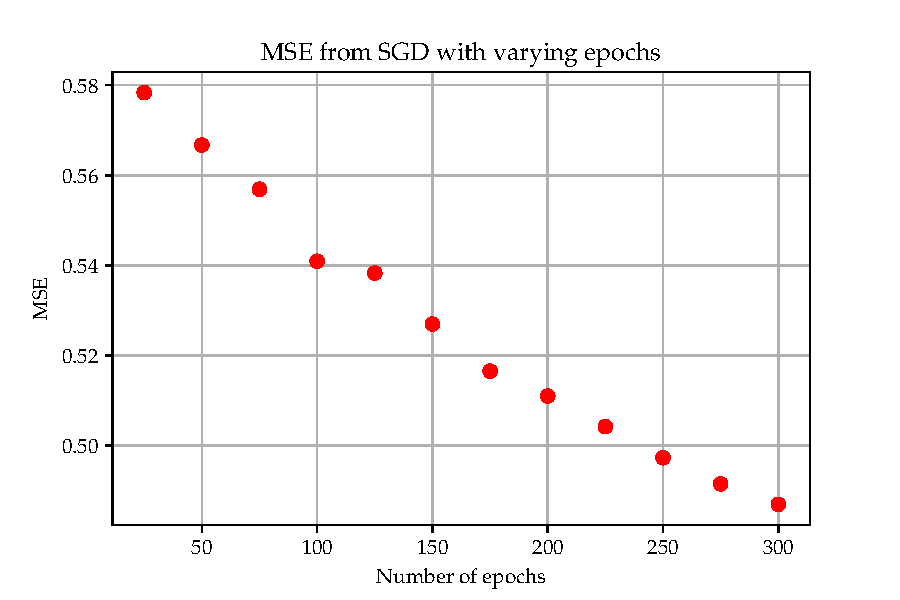
\includegraphics[width=\columnwidth]{figures/EX_A_mse_with_varying_epoch.pdf}
  \caption{\label{fig:a_mse_epoch}MSE calculated from Stochastic Gradient Descent optimization of the predictors $\theta$ as function of the number of epochs with all other hyperparameters kept fixed}
\end{figure}

\begin{table}
  \caption{\label{tab:a_epoch_run}Runtime in seconds computed for SGD over an increasing number of epochs}
  \begin{tabular}{|c|c|}
      \hline
      \#epochs & Runtime [s] \\ \hline
      25               & 8           \\ 
      50               & 17          \\ 
      75               & 27          \\ 
      100              & 38          \\ 
      125              & 45          \\ 
      150              & 57          \\ 
      175              & 65          \\ 
      200              & 80          \\ 
      225              & 78          \\ 
      250              & 79          \\ 
      275              & 88          \\ 
      300              & 95          \\
      \hline
  \end{tabular}
\end{table}

The following Figure (\ref{fig:a_gs}) plots the MSE as a function of batch\_size using the SGD algorithm in \ref{alg:sgd}. 

\begin{figure}
  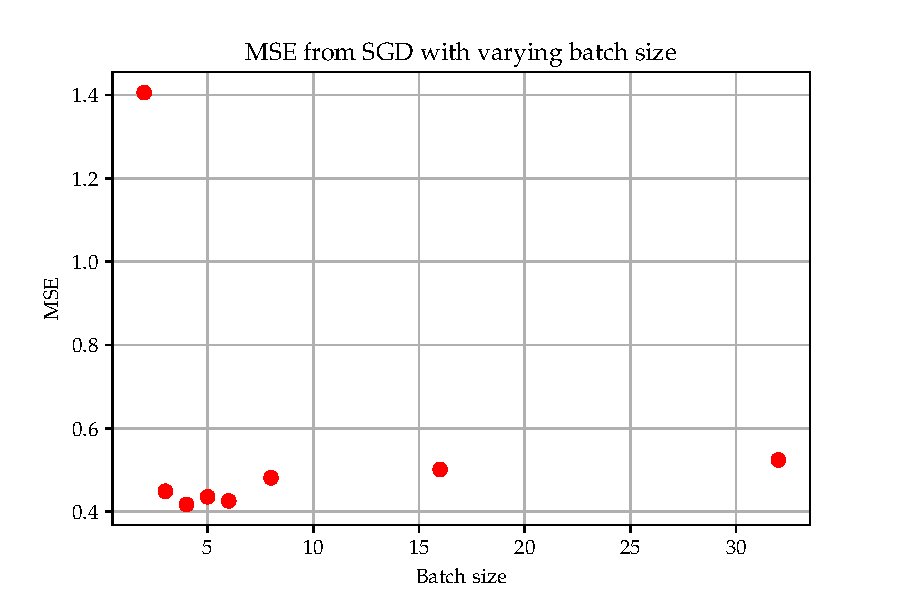
\includegraphics[width=\columnwidth]{figures/EX_A_mse_with_varying_batch_size.pdf}
  \caption{\label{fig:a_bs}MSE calculated from Stochastic Gradient Descent as function of the batch size with all other hyperparameters kept fixed}
\end{figure}

Both Figures (\ref{fig:a_gs}, \ref{fig:a_gslr}) are created using a grid search algorithm over different values of $\eta$ and $\lambda$, presented as a heatmap. 

\begin{figure*}
  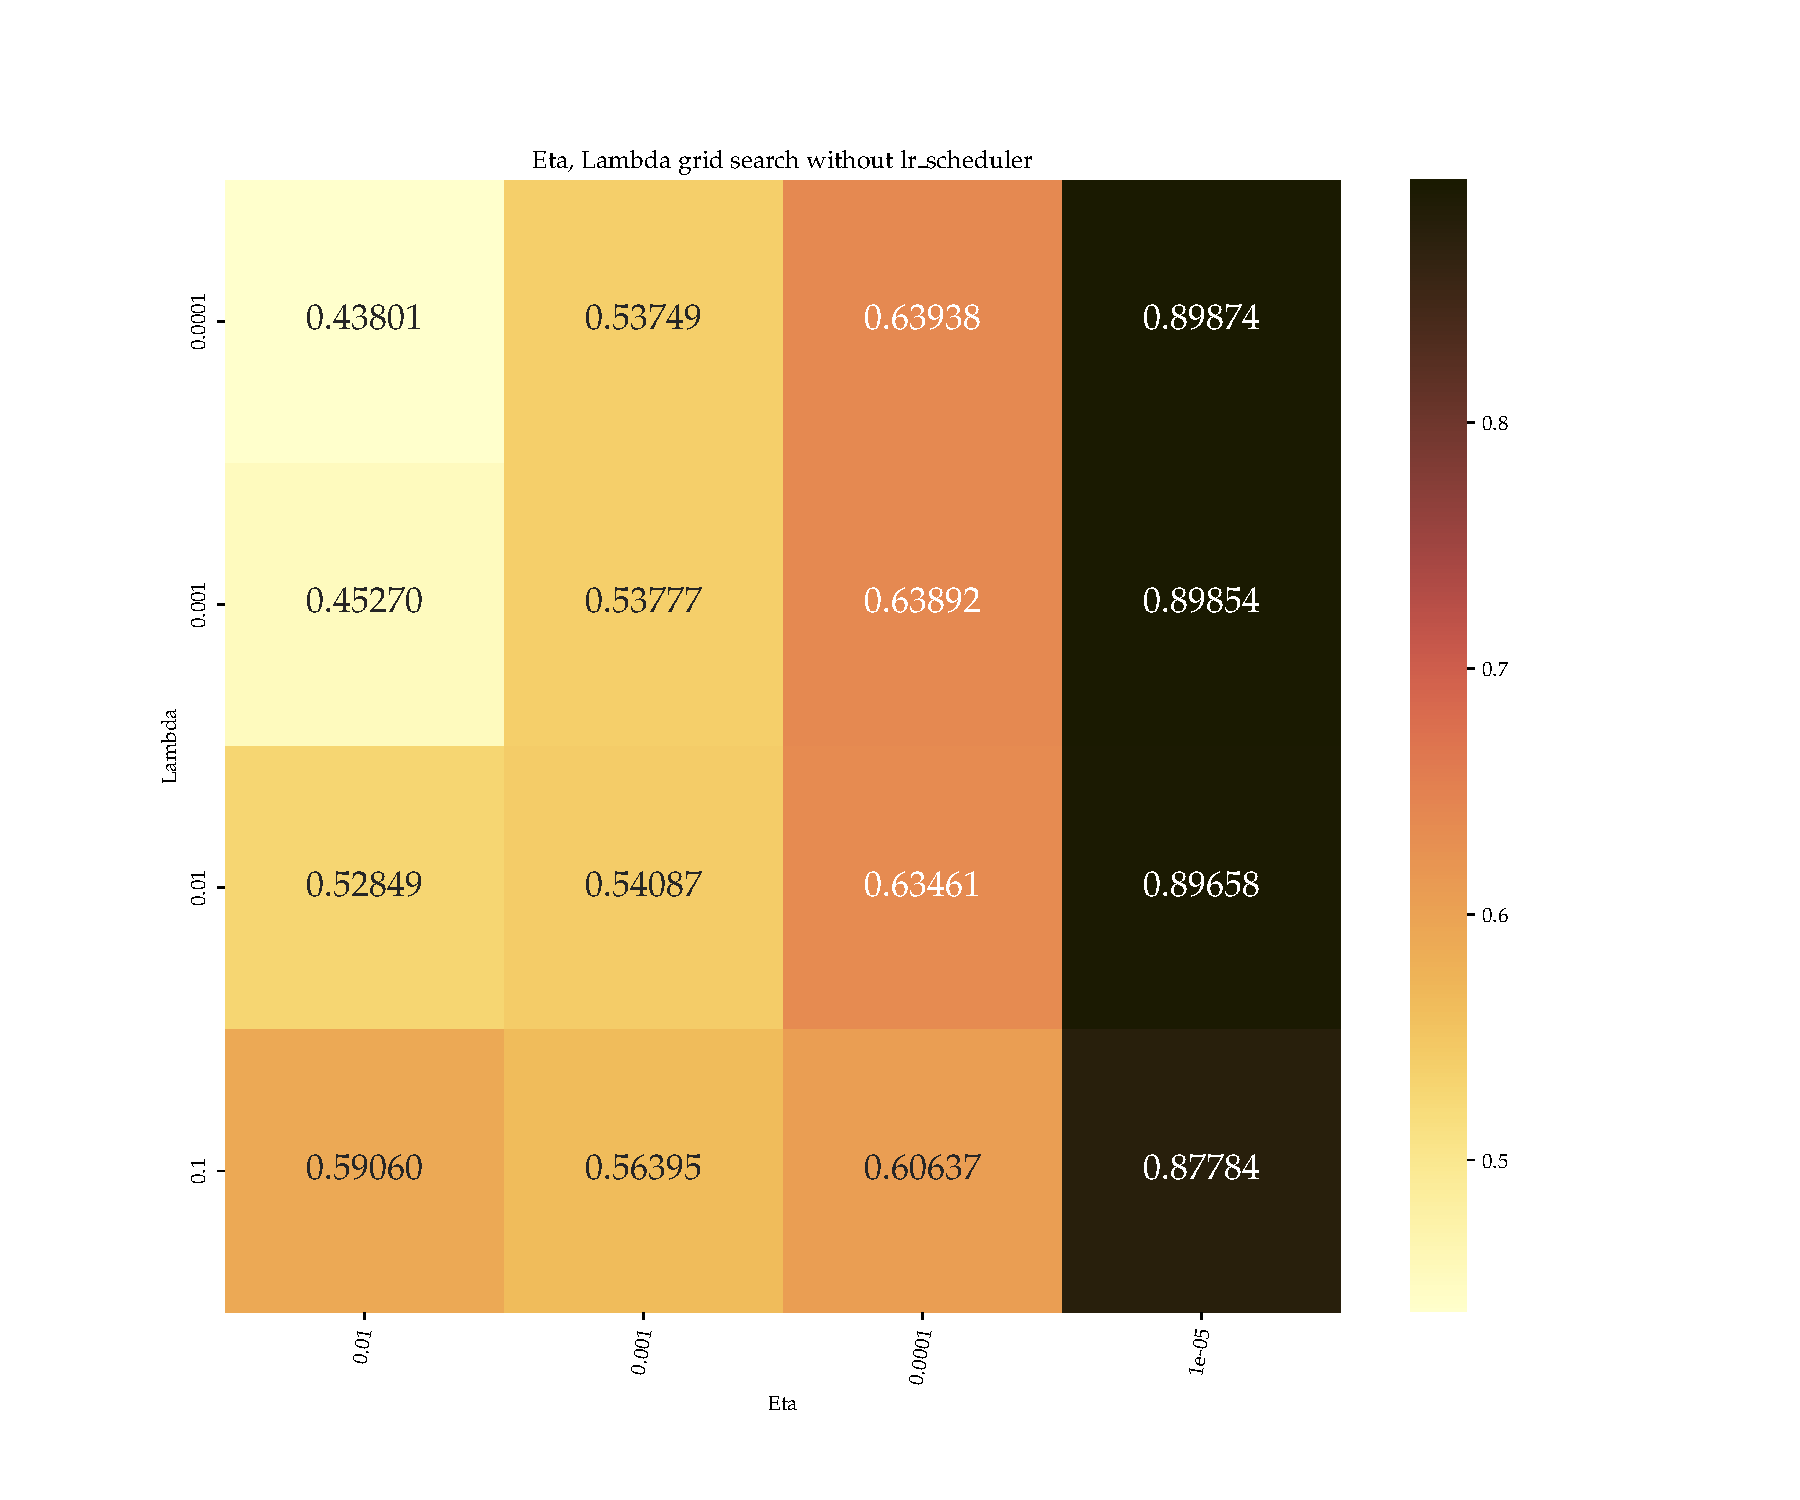
\includegraphics[width=\textwidth]{figures/EX_A__gridsearch.pdf}
  \caption{\label{fig:a_gs}MSE calculated for varying $\eta$ and $\lambda$ values in a grid search with learning rate scheduler turned off}
\end{figure*}

\begin{figure*}
  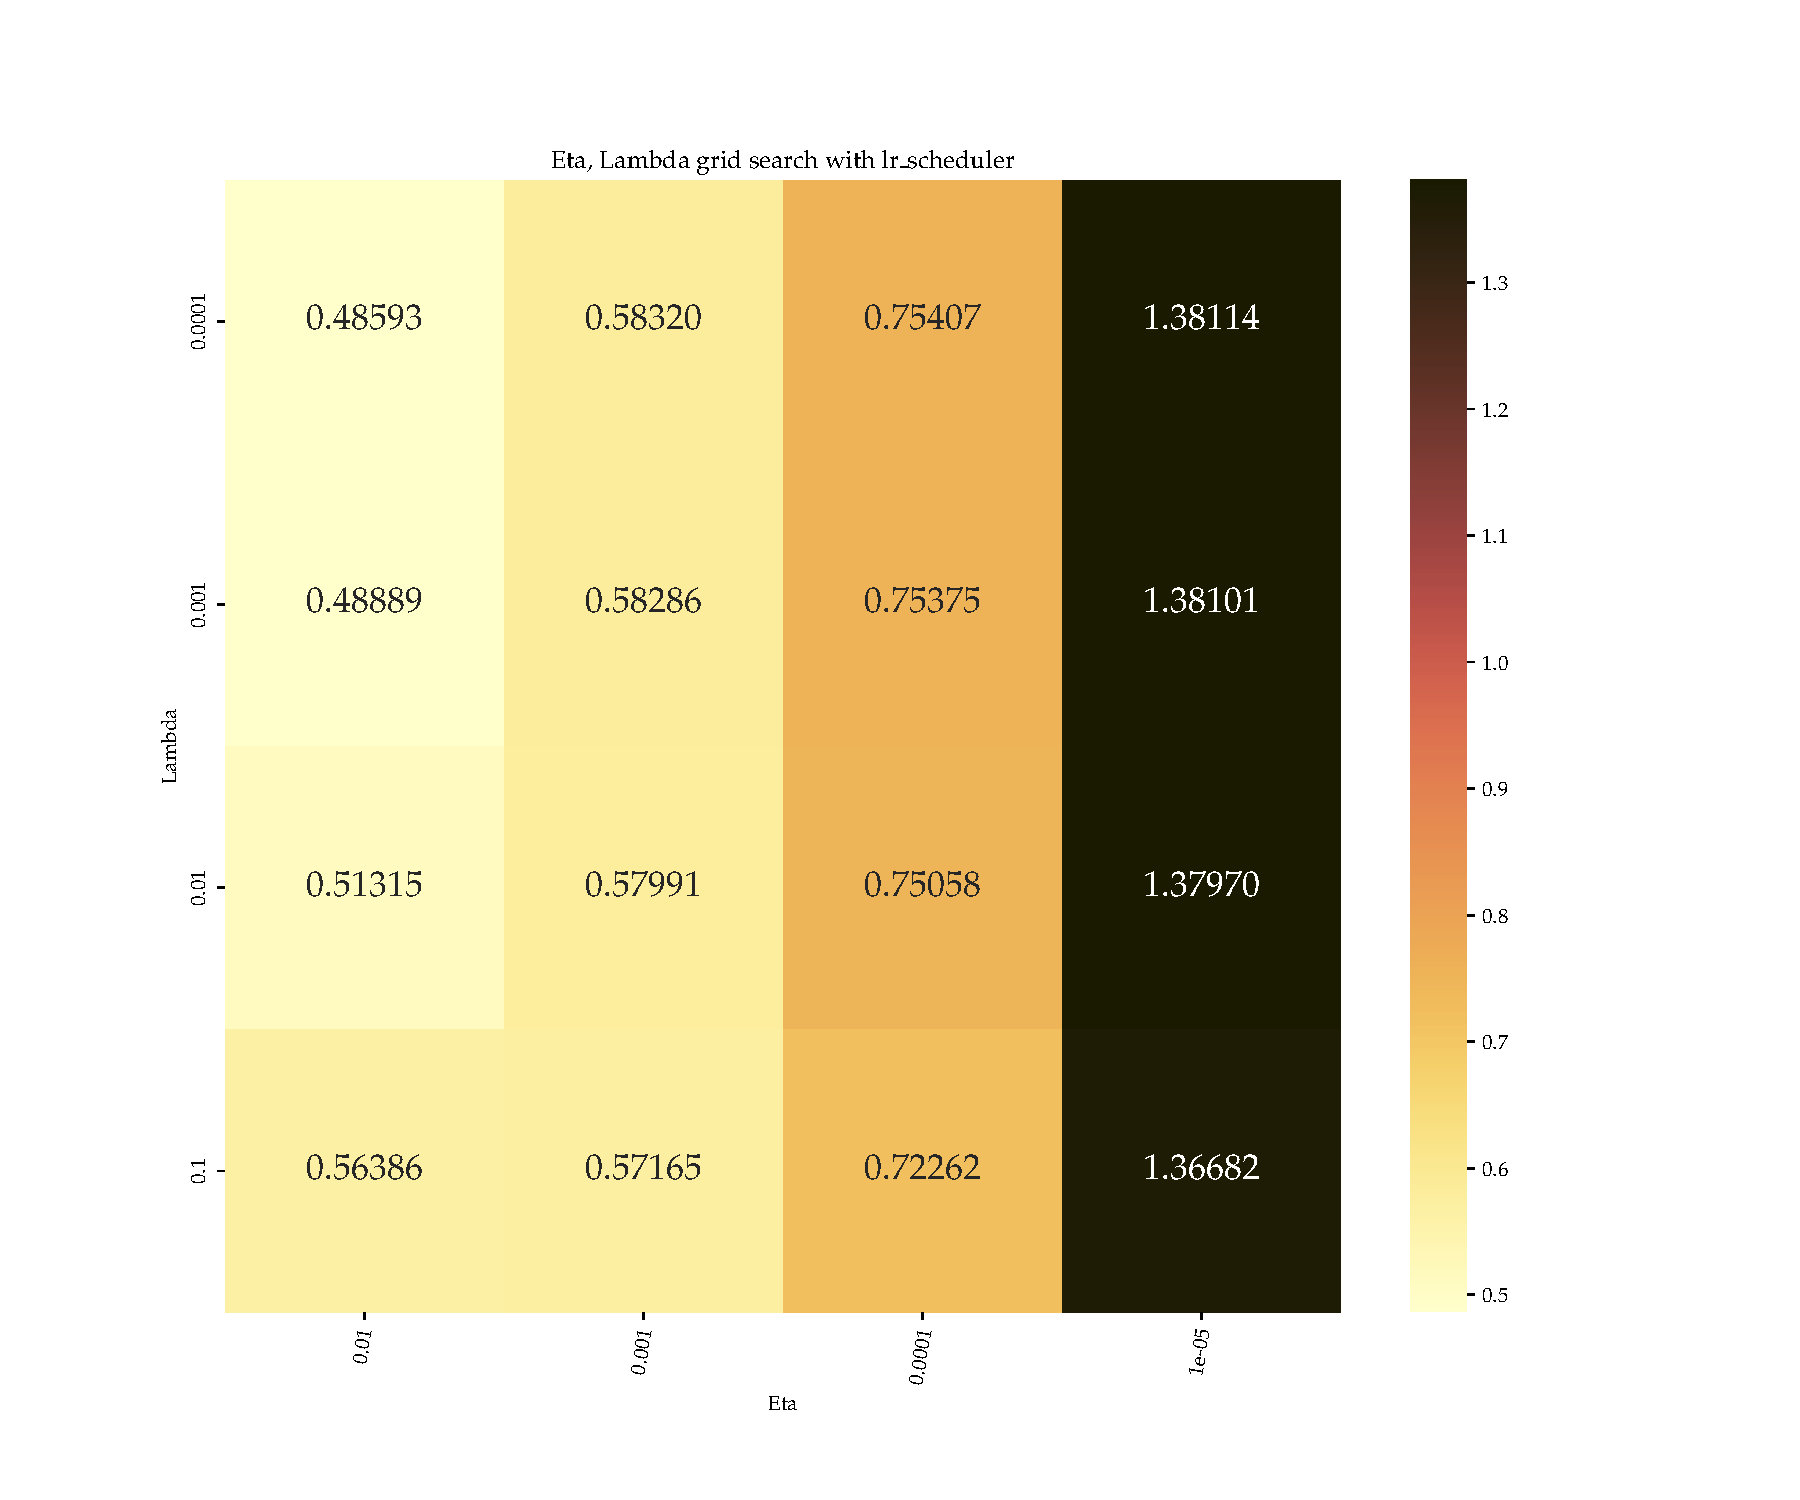
\includegraphics[width=\textwidth]{figures/EX_A__gridsearch_withlr.pdf}
  \caption{\label{fig:a_gslr}MSE calculated for varying $\eta$ and $\lambda$ values in a grid search with learning rate scheduler turned on}
\end{figure*}

Table (\ref{tab:a_mse}) displays MSE results computed from different configurations of the developed SGD algorithm as well as the MSE computed from the Momentum Stochastic Gradient Descent algorithm explained in Algorithm (\ref{alg:msgd}). 

\begin{table*}
  \caption{\label{tab:a_mse}MSE values from different SGD configurations based on the optimal hyperparameters as found in the grid search}
  \begin{ruledtabular}
    \begin{tabular}{lllll}
      SGD with lr scheduler & Momentum SGD with lr scheduler & SGD w.o. lr scheduler & SciKit-learn & Ridge\\
      \hline
      0.4783 & 0.4377 & 0.4203 & 1.0764 & 0.3256\\
    \end{tabular}
  \end{ruledtabular}
\end{table*}

\begin{table*}
  \caption{\label{tab:a_mse_lrlmb}MSE values from different SGD configurations based on the optimal hyperparameters as found in the grid search, without regularization}
  \begin{ruledtabular}
    \begin{tabular}{lllll}
      SGD with lr scheduler & Momentum SGD with lr scheduler & SGD w.o. lr scheduler & SciKit-learn & OLS\\
      \hline
      0.4778 & 0.4354 & 0.4171 & 1.0869 & 0.3216\\
    \end{tabular}
  \end{ruledtabular}
\end{table*}


\section{Discussion}
\subsection{Analyzing our Stochastic Gradient Descent implementation}
As described in the introduction, all results above are generated using the Terrain data from Project 1 with the same data preprocessing and a fixed degree of 6. The degree was chosen as a compromise between complexity to the data and complexity to the computations.
Figure (\ref{fig:a_mse_epoch}) shows the epoch dependance of the SGD algorithm measured in MSE. As can be seen in the figure, as the number of epochs are increased, the MSE is reduced. In this specific case, the reduction of MSE tend to closely follow a parabola, though for 100 epochs the MSE is reduced somewhat more than average. As such, the MSE seem to converge somewhere around 0.48, which is the approximate value at 300 epochs. However, though it can clearly be seen that a higher amount of epochs results in a more precise estimation of the predictors, the computational time for each run increases with epochs as seen in Table (\ref{tab:a_epoch_run}). Hence, as a consequence of running some of the computations on an Intel(R) Core(TM) i5-3230M CPU @ 2.60GHz, the number of epochs are constrained to 100 for further computations. Though we acknowledge that 100 epochs are not necessarily the optimal number of epochs if just concerning the MSE.  

Inspecting Figure (\ref{fig:a_bs}), it can be clearly seen that the lowest MSE values are attained for a batch size around 3 to 6 samples per batch. For batch sizes 8 and larger, the MSE tend to continuously increase following a weak slope. On the other hand, reducing the batch size to 2 samples per batch severely increases the MSE. Furthermore, for a batch size of 1 sample per batch, the MSE is not returned to due computational overflow (not shown). By combining the results of Figure (\ref{fig:a_mse_epoch}) and (\ref{fig:a_bs}), we can conclude that Stochastic Gradient Descent on the Terrain data performs optimal if given a descent number of epochs and a batch size of approximately 4. However, as previously discussed concerning computational resources, we have considered 100 epochs with a batch size of 4 the optimal when generating the coming results. 

The two heatmaps shown in Figures (\ref{fig:a_gs}) and (\ref{fig:a_gslr}) show the effect of the learning rate $\eta$ as well as the l2 regularization term $\lambda$ without and with a learning rate scheduler respectively. By comparing the two plots, it can be seen that the learning rate scheduler causes all but one model to attain higher MSE. Which might be a result of too aggressive scheduling.

Moreover, a secondary observation of the inclusion of the learning rate can be pointed out. By comparing the two rightmost columns of Figure (\ref{fig:a_gs}) and (\ref{fig:a_gslr}), it can be seen that SGD differ greatly in MSE value for $\eta=0.00001$ regardless of regularization parameter. This might be an effect of scheduling the learning rate, in combination with the learning rate being initialized to such a low value that the model is unable converge in time of the scheduling reducing all movement along the gradient. Furthermore, the difference in MSE between the model for higher learning rates is not as great as for $\eta = 0.00001$, which then might be a result of the model reaching close to a minima before scheduling.

Figure (\ref{fig:a_gs}) shows that the optimal hyperparameters for our SGD algorithm given the current dataset, is $\eta = 0.01$ and $\lambda = 0.0001$. As such, Figure (\ref{fig:a_gs}) suggests that less regularization leads to lower attained MSE. This complies with the results of Table (\ref{tab:a_mse_lrlmb}), were an even lower MSE value is attained when noe regularization is present. Furthermore, by comparing the Ridge regression value in Table (\ref{tab:a_mse}) with the OLS value in Table (\ref{tab:a_mse_lrlmb}) it can be seen that OLS scores better than Ridge regression for the optimal regularization parameter as found in Figure (\ref{fig:a_gs}). These results are in line with what we discovered in Project 1 when analyzing our Ridge Regression algorithm and OLS algorithm on the same Terrain data, namely that OLS scores better in regards to MSE than Ridge.

By comparing the values in Table (\ref{tab:a_mse}), it can be seen that 
the MSE values computed with our SGD algorithm gets close to the Ridge regression value, with an approximate difference of 0.1 for SGD without learning rate scheduler. Moreover, our SGD outperforms that of SciKit-learn, which is more than doubled of our computed MSE values. The same trends can be seen for the OLS case in Table (\ref{tab:a_mse_lrlmb}). Our SGD algorithm outperforms that of SciKit-learn, though lower MSE values are achieved as discussed in the previous paragraph.

Another note when discussing Table (\ref{tab:a_mse}) and (\ref{tab:a_mse_lrlmb}) is the inclusion of Momentum SGD as described in Algorithm (\ref{alg:msgd}). With the added momentum parameter, lower MSE values are attained as all the hyperparameters are kept the same. Though the values are not as good as normal SGD without the learning rate scheduler.








\section{Conclusions}

\appendix

\section{Source Code}
\label{sec:sc} 
Link to github repository containing all developed code for this project: \url{https://github.com/AndreasBordvik/FYS-STK4155-Prj2_report}

% Create the reference section using BibTeX:

% ------------------- end of main content ---------------

\bibliographystyle{plain}
\bibliography{biblio}




\end{document}